\chapter{रासायनिक अभिक्रियाएँ: अभिकारक और उत्पाद}\label{ch:g7:chemical-reactions}

बारबेक्यू में लकड़ी का कोयला दहकता है। एक घंटे बाद काले टुकड़ों में से लगभग
कुछ नहीं बचता --- थोड़ी-सी धूसर राख, और वह ऊष्मा जिसने खाना पकाया। काला
कार्बन कहाँ गया? वह ग़ायब नहीं हुआ: वह \omterm{def:g4:air-a-mixture-of-gases:air}{वायु} की ऑक्सीजन से मिला और एक नई,
अदृश्य गैस बन गया। \omterm{def:g7:atoms-and-molecules:atom}{परमाणु} और \omterm{def:g7:atoms-and-molecules:molecule}{अणु} हाथ में आ जाने पर अब हम ठीक-ठीक बता सकते
हैं कि ऐसे परिवर्तन में क्या होता है।

\begin{recall}
\omterm{def:g5:irreversible-changes:chemical-change}{रासायनिक परिवर्तन} में नए पदार्थ प्रकट होते हैं और वापसी का कोई सीधा रास्ता
नहीं होता (\cref{ch:g5:irreversible-changes})। चूने का पानी कार्बन
डाइऑक्साइड से दूधिया हो जाता है, निर्जल कॉपर सल्फ़ेट पानी से नीला
(\cref{ch:g7:identifying-substances})। सारा द्रव्य \omterm{def:g7:atoms-and-molecules:atom}{परमाणुओं} से बना है,
जो मिलकर \omterm{def:g7:atoms-and-molecules:molecule}{अणु} बनाते हैं; \ce{CO2} जैसा सूत्र किसी \omterm{def:g7:atoms-and-molecules:molecule}{अणु} के \omterm{def:g7:atoms-and-molecules:atom}{परमाणुओं} की सूची
देता है (\cref{ch:g7:atoms-and-molecules})।
\end{recall}

\begin{omfigure}
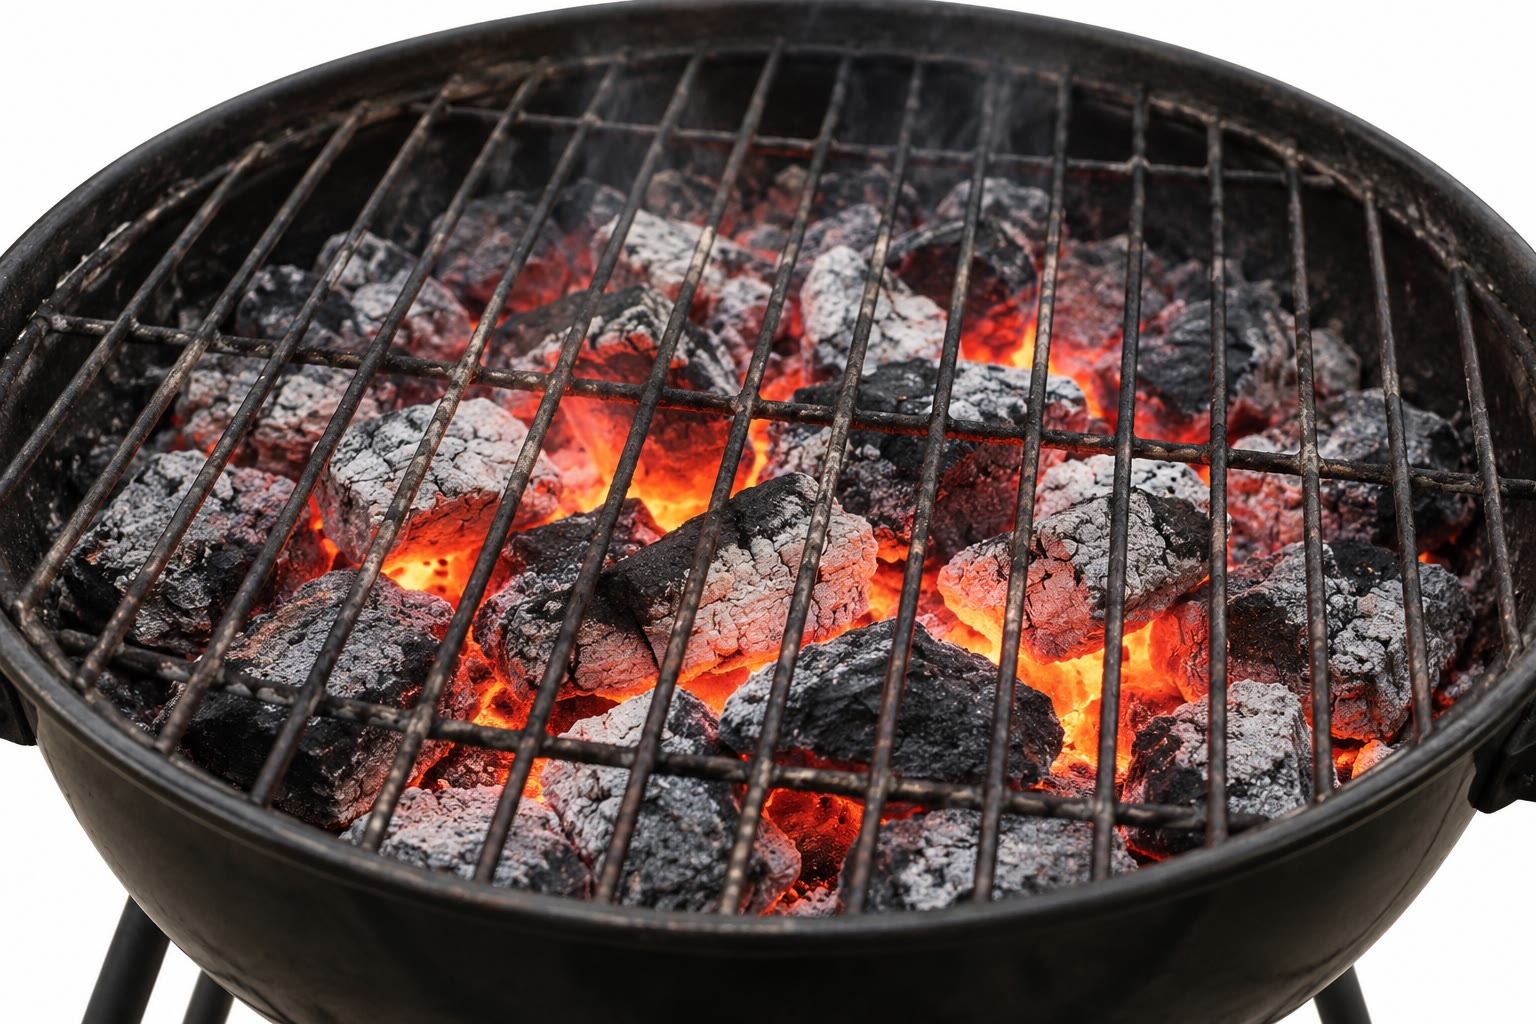
\includegraphics[width=0.55\linewidth]{images/book1/ai/g7-charcoal-bbq.jpg}

{\small दहकता कोयला: कार्बन \omterm{def:g4:air-a-mixture-of-gases:air}{वायु} की ऑक्सीजन के साथ अभिक्रिया कर रहा है।}
\end{omfigure}

\section{भौतिक और रासायनिक रूपांतरण}

\begin{definition}[भौतिक रूपांतरण]\label{def:g7:chemical-reactions:physical-transformation}
\emph{भौतिक रूपांतरण}\index{भौतिक रूपांतरण} \omterm{def:g6:pure-substances-and-mixtures:species}{रासायनिक स्पीशीज़} को
बदले बिना द्रव्य की अवस्था या उसकी व्यवस्था को बदलता है: पिघलना, जमना,
उबलना, \omterm{def:g2:mixing-and-dissolving:dissolve}{घुलना}, \omterm{def:g2:mixing-and-dissolving:mix}{मिलाना}। पहले और बाद में वही स्पीशीज़ मौजूद रहती हैं;
केवल उनका रूप या उनकी व्यवस्था बदली है।
\end{definition}

\begin{example}[पानी, तीन तरह से]\label{ex:g7:chemical-reactions:water}
बर्फ़ का पिघलकर पानी बनना, पानी का उबलकर जलवाष्प बनना, और पानी में नमक का
\omterm{def:g2:mixing-and-dissolving:dissolve}{घुलना} \omterm{def:g7:chemical-reactions:physical-transformation}{भौतिक रूपांतरण} हैं: पहले और बाद में पानी के \omterm{def:g7:atoms-and-molecules:molecule}{अणु} (और नमक)
मौजूद हैं। बहुत आवर्धन करके देखें, तो \omterm{def:g7:atoms-and-molecules:molecule}{अणु} वही हैं; केवल उनकी व्यवस्था और
उनकी गति बदली है।
\end{example}

\begin{proposition}[रासायनिक रूपांतरण]\label{prop:g7:chemical-reactions:chemical}
\omterm{def:g5:irreversible-changes:chemical-change}{रासायनिक परिवर्तन} में, जिसे रासायनिक रूपांतरण भी कहते हैं, कुछ \omterm{def:g6:pure-substances-and-mixtures:species}{रासायनिक
स्पीशीज़} ग़ायब होती हैं और नई प्रकट होती हैं। \omterm{def:g7:chemical-reactions:physical-transformation}{भौतिक रूपांतरण} से इसे इसके
उत्पादों से अलग पहचाना जाता है: नई स्पीशीज़, जिन्हें \omterm{def:g7:identifying-substances:characteristic-test}{अभिलाक्षणिक परीक्षणों} से
पहचाना जा सकता है।
\end{proposition}

\begin{omfigure}
\begin{tikzpicture}[font=\small, level distance=1.5cm,
    box/.style={draw=omDef, fill=omDef!6, rounded corners=2pt, align=center,
      inner sep=4pt},
    level 1/.style={sibling distance=6.6cm},
    edge from parent/.style={draw, thick, omDef, ->}]
  \node[box] {द्रव्य का एक रूपांतरण}
    child {node[box, text width=5.2cm] {\textbf{भौतिक}: पहले और बाद में\\
      वही स्पीशीज़\\ \footnotesize पिघलना, उबलना, घुलना, मिलाना}}
    child {node[box, draw=omProp, fill=omProp!6, text width=5.2cm]
      {\textbf{रासायनिक}: स्पीशीज़ ग़ायब होती हैं,\\ नई स्पीशीज़ प्रकट होती हैं\\
      \footnotesize जलना, जंग लगना, पकाना}};
\end{tikzpicture}

{\small रूपांतरण के दो प्रकार।}
\end{omfigure}

\section{अभिकारक और उत्पाद}

\begin{definition}[रासायनिक अभिक्रिया]\label{def:g7:chemical-reactions:reaction}
\emph{रासायनिक अभिक्रिया}\index{रासायनिक अभिक्रिया} वह मॉडल है जिससे
रसायनज्ञ किसी रासायनिक रूपांतरण का वर्णन करते हैं: यह बताती है कि किन
स्पीशीज़ की खपत होती है और कौन-सी स्पीशीज़ बनती हैं।
\end{definition}

\begin{definition}[अभिकारक और उत्पाद]\label{def:g7:chemical-reactions:reactant}
किसी \omterm{def:g7:chemical-reactions:reaction}{रासायनिक अभिक्रिया} में जिन स्पीशीज़ की खपत होती है, वे
\emph{अभिकारक}\index{अभिकारक} हैं; जो स्पीशीज़ बनती हैं, वे
\emph{उत्पाद}\index{उत्पाद} हैं।
\end{definition}

\begin{example}[ऑक्सीजन में कार्बन का जलना]\label{ex:g7:chemical-reactions:carbon}
जब लकड़ी का कोयला \omterm{def:g4:what-a-fire-needs:burning}{जलता} है, तो \omterm{def:g7:chemical-reactions:reactant}{अभिकारक} कार्बन (कोयला) और ऑक्सीजन
(\omterm{def:g4:air-a-mixture-of-gases:air}{वायु} से) होते हैं। \omterm{def:g7:chemical-reactions:reactant}{उत्पाद} कार्बन डाइऑक्साइड है: जार में बची गैस को चूने के
पानी के साथ हिलाने पर वह दूधिया हो जाता है।
\end{example}

\begin{inthelab}[ऑक्सीजन के जार में कोयला]
शिक्षक एक \omterm{def:g4:what-a-fire-needs:burning}{दहन} चम्मच पर कोयले के एक छोटे टुकड़े को दहकने तक गरम करते हैं,
फिर उसे ऑक्सीजन के जार में उतारते हैं। कोयला \omterm{def:g4:air-a-mixture-of-gases:air}{वायु} की तुलना में कहीं
ज़्यादा चमक से दहकता है और सिकुड़ते-सिकुड़ते ख़त्म हो जाता है। जार को ढककर
उसमें थोड़ा चूने का पानी डालकर हिलाया जाता है: वह दूधिया हो जाता है।
कार्बन और ऑक्सीजन की खपत हुई है; कार्बन डाइऑक्साइड बनी है।
\end{inthelab}

\begin{omfigure}
\begin{tikzpicture}[font=\small, scale=1.3]
  \pic[transform shape] at (0,0) {gasjaropen={0}{white}};
  \fill[omWater!60] (-0.68,2.62) rectangle (0.68,2.7);
  \draw[omGlass, line width=0.4pt] (-0.68,2.62) rectangle (0.68,2.7);
  \draw[black!60, line width=1.2pt] (0.15,2.7) -- (0.15,3.6) -- (1.2,3.6);
  \draw[black!60, line width=1.2pt] (0.15,2.7) -- (0.15,1.2);
  \fill[black!60] (-0.12,1.12) rectangle (0.32,1.2);
  \fill[red!70!black] (0.0,1.32) circle (0.13);
  \fill[orange!90!yellow] (0.0,1.32) circle (0.08);
  \draw[<-, omProp, thick] (0.15,1.35) -- (1.5,1.6) node[right, text=black]
    {दहकता कोयला (कार्बन)};
  \draw[<-, omProp, thick] (-0.35,2.1) -- (1.5,2.3) node[right, text=black]
    {ऑक्सीजन};
  \draw[<-, omProp, thick] (0.6,2.66) -- (1.5,2.95) node[right, text=black]
    {ढक्कन};
  \draw[<-, omProp, thick] (0.15,3.1) -- (1.5,3.6) node[right, text=black]
    {दहन चम्मच};
\end{tikzpicture}

{\small चम्मच पर रखकर ऑक्सीजन के जार में उतारा गया दहकता कोयला तेज़ चमक से
\omterm{def:g4:what-a-fire-needs:burning}{जलता} है: कार्बन और ऑक्सीजन अभिक्रिया करके कार्बन डाइऑक्साइड बनाते हैं।}
\end{omfigure}

\begin{example}[स्टील ऊन]\label{ex:g7:chemical-reactions:steel-wool}
बारीक स्टील ऊन का एक गुच्छा, जो ज़्यादातर लोहा है, \omterm{def:g4:air-a-mixture-of-gases:air}{वायु} में चिंगारियों की
बौछार के साथ जल सकता है। \omterm{def:g7:chemical-reactions:reactant}{अभिकारक} लोहा और ऑक्सीजन हैं; \omterm{def:g7:chemical-reactions:reactant}{उत्पाद} एक गहरे
रंग का, भुरभुरा ठोस है, एक आयरन ऑक्साइड।
\end{example}

\begin{omfigure}
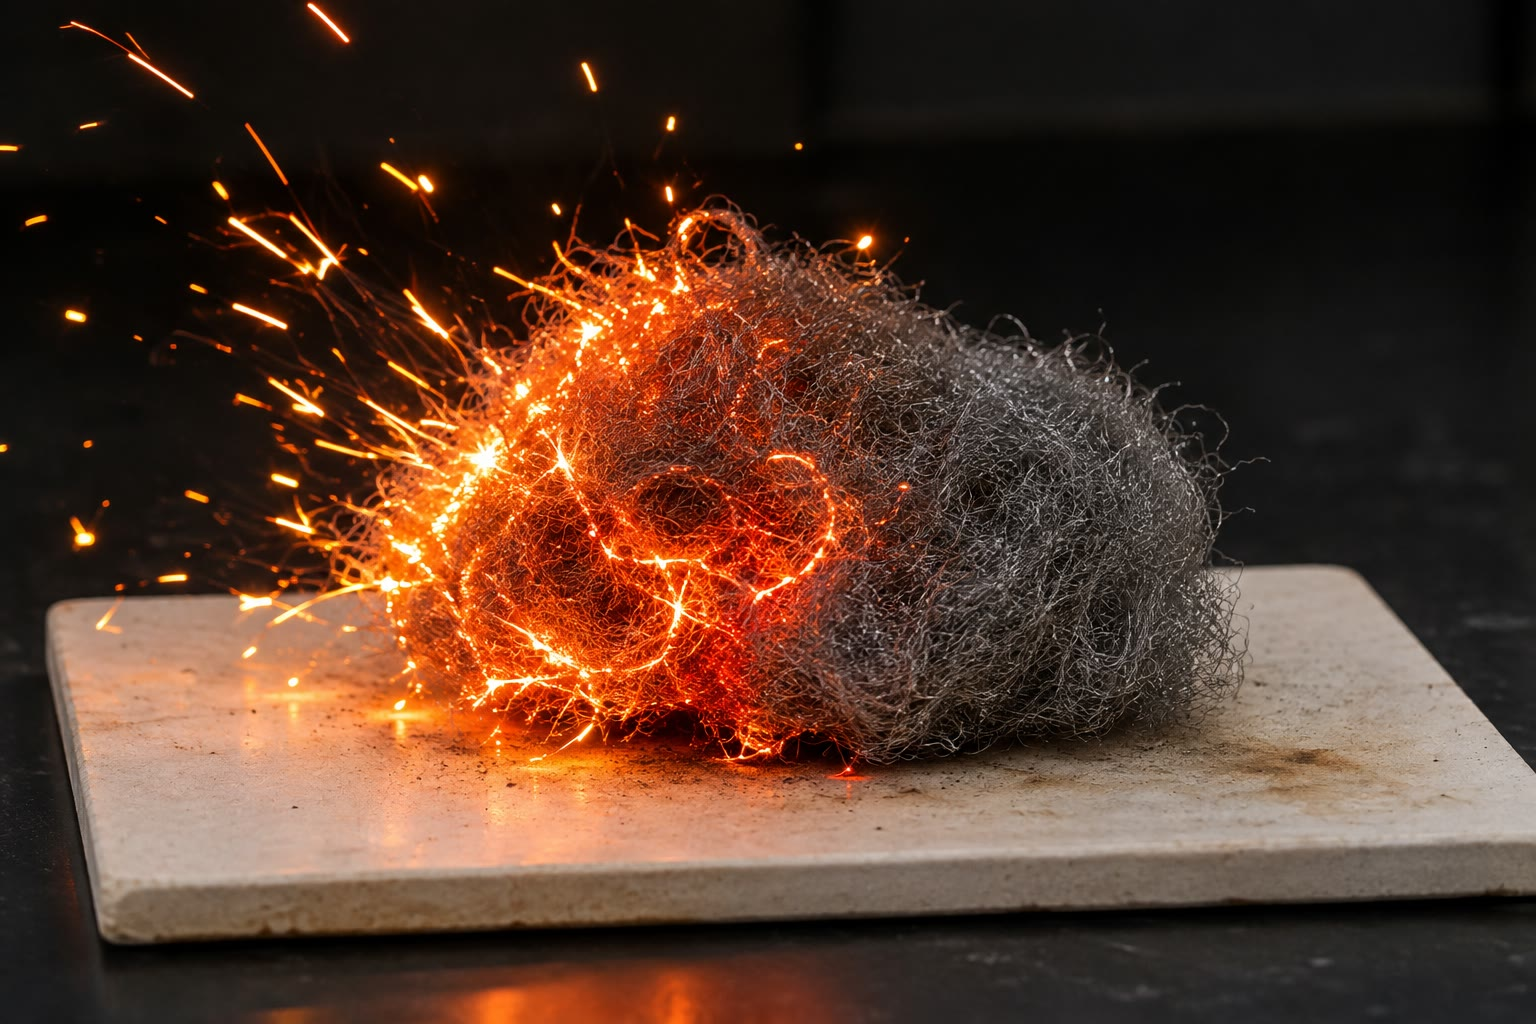
\includegraphics[width=0.5\linewidth]{images/book1/ai/g7-steel-wool-burning.jpg}

{\small प्रयोगशाला में \omterm{def:g4:what-a-fire-needs:burning}{जलती} स्टील ऊन: लोहा और ऑक्सीजन अभिक्रिया करते हैं।}
\end{omfigure}

\section{शाब्दिक समीकरण}

\begin{definition}[शाब्दिक समीकरण]\label{def:g7:chemical-reactions:word-equation}
\emph{शाब्दिक समीकरण}\index{शाब्दिक समीकरण} किसी \omterm{def:g7:chemical-reactions:reaction}{रासायनिक अभिक्रिया} को
शब्दों में लिखता है: बाईं ओर \omterm{def:g7:chemical-reactions:reactant}{अभिकारकों} के नाम, $+$ से जुड़े हुए, फिर एक
तीर, और दाईं ओर उत्पादों के नाम। तीर को ``अभिक्रिया करके देते हैं''
पढ़ा जाता है।
\end{definition}

\begin{example}[तीन शाब्दिक समीकरण]\label{ex:g7:chemical-reactions:three}
\begin{center}
\begin{tabular}{l}
कार्बन $+$ ऑक्सीजन $\longrightarrow$ कार्बन डाइऑक्साइड\\[2pt]
मेथेन $+$ ऑक्सीजन $\longrightarrow$ कार्बन डाइऑक्साइड $+$ पानी\\[2pt]
लोहा $+$ ऑक्सीजन $\longrightarrow$ आयरन ऑक्साइड
\end{tabular}
\end{center}
\end{example}

\begin{method}[शाब्दिक समीकरण लिखना]\label{met:g7:chemical-reactions:write}
\begin{enumerate}
  \item \omterm{def:g7:chemical-reactions:reactant}{अभिकारक} पहचानो: वे स्पीशीज़ जो ग़ायब होती हैं।
  \item \omterm{def:g7:chemical-reactions:reactant}{उत्पाद} पहचानो: नई स्पीशीज़, जिन्हें परीक्षणों से पहचाना गया है।
  \item \omterm{def:g7:chemical-reactions:reactant}{अभिकारकों} को बाईं ओर, उत्पादों को दाईं ओर लिखो,
        बीच में एक तीर के साथ; बराबर का चिह्न कभी नहीं।
\end{enumerate}
जो स्पीशीज़ मौजूद है पर भाग नहीं लेती --- लौ के आस-पास की \omterm{def:g4:air-a-mixture-of-gases:air}{वायु} की
नाइट्रोजन --- वह लिखी नहीं जाती।
\end{method}

\section{अभिक्रिया परमाणुओं की नई व्यवस्था है}

\begin{proposition}[परमाणु नए ढंग से व्यवस्थित होते हैं]\label{prop:g7:chemical-reactions:rearranged}
\omterm{def:g7:chemical-reactions:reaction}{रासायनिक अभिक्रिया} में \omterm{def:g7:chemical-reactions:reactant}{अभिकारकों} के \omterm{def:g7:atoms-and-molecules:molecule}{अणु} टूटते हैं और उनके \omterm{def:g7:atoms-and-molecules:atom}{परमाणु} दूसरे ढंग
से जुड़कर उत्पादों के \omterm{def:g7:atoms-and-molecules:molecule}{अणु} बनाते हैं। \omterm{def:g7:atoms-and-molecules:atom}{परमाणु} स्वयं न बनते हैं, न नष्ट होते
हैं: पहले और बाद में वही \omterm{def:g7:atoms-and-molecules:atom}{परमाणु}, उतनी ही संख्या में,
मौजूद रहते हैं।
\end{proposition}

\begin{example}[मेथेन का जलना, अणु-दर-अणु]\label{ex:g7:chemical-reactions:methane}
जब गैस चूल्हे की मेथेन \omterm{def:g4:what-a-fire-needs:burning}{जलती} है, तो मेथेन का एक \omterm{def:g7:atoms-and-molecules:molecule}{अणु} \ce{CH4}
ऑक्सीजन के दो \omterm{def:g7:atoms-and-molecules:molecule}{अणुओं} \ce{O2} से मिलता है। उनके \omterm{def:g7:atoms-and-molecules:atom}{परमाणु} नए ढंग से व्यवस्थित होकर
कार्बन डाइऑक्साइड का एक \omterm{def:g7:atoms-and-molecules:molecule}{अणु} \ce{CO2} और पानी के दो \omterm{def:g7:atoms-and-molecules:molecule}{अणु} \ce{H2O} बना देते हैं।
पहले: 1 कार्बन, 4 हाइड्रोजन और 4 ऑक्सीजन \omterm{def:g7:atoms-and-molecules:atom}{परमाणु}। बाद में: 1 कार्बन, 4
हाइड्रोजन, और $2 + 2 = 4$ ऑक्सीजन \omterm{def:g7:atoms-and-molecules:atom}{परमाणु}। न कुछ खोता है, न कुछ
कहीं से प्रकट होता है।
\end{example}

\begin{omfigure}
\begin{tikzpicture}[font=\small]
  % methane
  \begin{scope}[xshift=0cm]
    \node[aC] (c) at (0,0) {};
    \node[aH] (h1) at (0,0.78) {}; \node[aH] (h2) at (-0.74,-0.3) {};
    \node[aH] (h3) at (0.74,-0.3) {}; \node[aH] (h4) at (0.2,-0.68) {};
    \begin{scope}[on background layer]
      \foreach \h in {h1,h2,h3,h4} \draw[bond] (c.center) -- (\h.center);
    \end{scope}
    \node at (0,-1.2) {1 मेथेन};
  \end{scope}
  \node at (1.45,0) {$+$};
  % two oxygen molecules
  \foreach \y in {0.45,-0.45} {
    \node[aO] (a) at (2.4,\y) {}; \node[aO] (b) at (3.05,\y) {};
    \begin{scope}[on background layer]
      \draw[bond, line width=1.1pt] ([yshift=1.6pt]a.center) -- ([yshift=1.6pt]b.center);
      \draw[bond, line width=1.1pt] ([yshift=-1.6pt]a.center) -- ([yshift=-1.6pt]b.center);
    \end{scope}
  }
  \node at (2.72,-1.2) {2 ऑक्सीजन};
  \draw[->, thick, omProp] (3.8,0) -- (5.0,0);
  % carbon dioxide
  \begin{scope}[xshift=6.3cm]
    \node[aO] (a) at (-0.8,0) {}; \node[aC] (c) at (0,0) {}; \node[aO] (b) at (0.8,0) {};
    \begin{scope}[on background layer]
      \foreach \d in {-1.6,1.6} {
        \draw[bond, line width=1.1pt] ([yshift=\d pt]a.center) -- ([yshift=\d pt]c.center);
        \draw[bond, line width=1.1pt] ([yshift=\d pt]c.center) -- ([yshift=\d pt]b.center);}
    \end{scope}
    \node at (0,-1.2) {1 कार्बन डाइऑक्साइड};
  \end{scope}
  \node at (7.8,0) {$+$};
  % two water molecules
  \foreach \x in {8.9,10.6} {
    \node[aO] (o) at (\x,0.2) {};
    \node[aH] (p) at (\x-0.58,-0.25) {}; \node[aH] (q) at (\x+0.58,-0.25) {};
    \begin{scope}[on background layer]
      \draw[bond] (o.center) -- (p.center); \draw[bond] (o.center) -- (q.center);
    \end{scope}
  }
  \node at (9.75,-1.2) {2 पानी};
  % atom counts
  \node[align=center, font=\footnotesize] at (1.5,-2.0) {पहले: 1 C, 4 H, 4 O};
  \node[align=center, font=\footnotesize] at (8.5,-2.0) {बाद में: 1 C, 4 H, 4 O};
\end{tikzpicture}

{\small आण्विक मॉडलों से बनाया गया मेथेन का \omterm{def:g4:what-a-fire-needs:burning}{जलना}: \omterm{def:g7:chemical-reactions:reactant}{अभिकारकों} के \omterm{def:g7:atoms-and-molecules:atom}{परमाणु} नए
ढंग से व्यवस्थित होकर \omterm{def:g7:chemical-reactions:reactant}{उत्पाद} बनते हैं। पहले और बाद में वही \omterm{def:g7:atoms-and-molecules:atom}{परमाणु}
गिने जाते हैं।}
\end{omfigure}

\begin{remark}[अणुओं को गिनना]\label{rem:g7:chemical-reactions:counting}
\omterm{def:g7:chemical-reactions:word-equation}{शाब्दिक समीकरण} यह नहीं बताता कि कितने \omterm{def:g7:atoms-and-molecules:molecule}{अणु} अभिक्रिया करते हैं: इसके लिए
समीकरण सूत्रों से, और उनके आगे संख्याएँ लगाकर, लिखा जाता है। ऐसे समीकरण लिखना,
और सही संख्याएँ खोजना, आगे के एक अध्याय का
विषय है।
\end{remark}

\section{अभ्यास}

\begin{exercise}[$\star$]\label{exo:g7:chemical-reactions:1}
भौतिक या रासायनिक रूपांतरण? बर्फ़ का पिघलना, तीली का \omterm{def:g4:what-a-fire-needs:burning}{जलना}, चीनी का
\omterm{def:g2:mixing-and-dissolving:dissolve}{घुलना}, डबलरोटी का सिंकना, कील में जंग लगना।
\end{exercise}

\begin{exercise}[$\star$]\label{exo:g7:chemical-reactions:2}
किसी \omterm{def:g7:chemical-reactions:reaction}{रासायनिक अभिक्रिया} के \omterm{def:g7:chemical-reactions:reactant}{अभिकारक} और \omterm{def:g7:chemical-reactions:reactant}{उत्पाद} क्या होते हैं?
\end{exercise}

\begin{exercise}[$\star$]\label{exo:g7:chemical-reactions:3}
ऑक्सीजन में कार्बन के \omterm{def:g4:what-a-fire-needs:burning}{जलने} का \omterm{def:g7:chemical-reactions:word-equation}{शाब्दिक समीकरण} लिखो।
\end{exercise}

\begin{exercise}[$\star$]\label{exo:g7:chemical-reactions:4}
\omterm{def:g7:chemical-reactions:word-equation}{शाब्दिक समीकरण} ``लोहा $+$ ऑक्सीजन $\longrightarrow$ आयरन ऑक्साइड'' में
\omterm{def:g7:chemical-reactions:reactant}{अभिकारकों} और \omterm{def:g7:chemical-reactions:reactant}{उत्पाद} के नाम बताओ।
\end{exercise}

\begin{exercise}[$\star\star$]\label{exo:g7:chemical-reactions:5}
मेथेन के \omterm{def:g4:what-a-fire-needs:burning}{जलने} पर लौ के ऊपर पकड़ा गया ठंडा गिलास धुँधला हो जाता है, और
इकट्ठी की गई गैस चूने के पानी को दूधिया कर देती है। ये दोनों परीक्षण कौन-से
\omterm{def:g7:chemical-reactions:reactant}{उत्पाद} दिखाते हैं?
\end{exercise}

\begin{exercise}[$\star\star$]\label{exo:g7:chemical-reactions:6}
ज़िंक हाइड्रोक्लोरिक अम्ल के साथ अभिक्रिया करता है: ज़िंक ग़ायब हो जाता है,
हाइड्रोजन के बुलबुले निकलते हैं, और ज़िंक क्लोराइड विलयन में रह जाता है।
\omterm{def:g7:chemical-reactions:word-equation}{शाब्दिक समीकरण} लिखो।
\end{exercise}

\begin{exercise}[$\star\star$]\label{exo:g7:chemical-reactions:7}
मेथेन के \omterm{def:g4:what-a-fire-needs:burning}{जलने} वाला मॉडल-चित्र देखो। अभिक्रिया से पहले और बाद में
हाइड्रोजन \omterm{def:g7:atoms-and-molecules:atom}{परमाणु} गिनो।
\end{exercise}

\begin{exercise}[$\star\star$]\label{exo:g7:chemical-reactions:8}
पानी में नमक घोलना \omterm{def:g7:chemical-reactions:reaction}{रासायनिक अभिक्रिया} क्यों नहीं है, हालाँकि नमक आँखों से
ओझल हो जाता है?
\end{exercise}

\begin{exercise}[$\star\star$]\label{exo:g7:chemical-reactions:9}
लकड़ी का एक लट्ठा जलकर राख की छोटी-सी ढेरी रह जाता है। ``\omterm{def:g7:chemical-reactions:reactant}{उत्पाद}'' शब्द का
उपयोग करके समझाओ कि राख लट्ठे से इतनी हल्की क्यों है।
\end{exercise}

\begin{exercise}[$\star\star$]\label{exo:g7:chemical-reactions:10}
हाइड्रोजन ऑक्सीजन में जलकर केवल पानी देती है। \omterm{def:g7:chemical-reactions:word-equation}{शाब्दिक समीकरण} लिखो,
और बताओ कि \omterm{def:g7:chemical-reactions:reactant}{उत्पाद} को कौन-सा परीक्षण पहचानेगा।
\end{exercise}

\begin{exercise}[$\star\star\star$]\label{exo:g7:chemical-reactions:11}
हाइड्रोजन के दो \omterm{def:g7:atoms-and-molecules:molecule}{अणु} \ce{H2} ऑक्सीजन के एक \omterm{def:g7:atoms-and-molecules:molecule}{अणु} \ce{O2} के साथ अभिक्रिया
करके पानी के दो \omterm{def:g7:atoms-and-molecules:molecule}{अणु} \ce{H2O} देते हैं। पहले और बाद में हर प्रकार के \omterm{def:g7:atoms-and-molecules:atom}{परमाणु}
गिनो, और दिखाओ कि कोई भी न बना है, न नष्ट हुआ है।
\end{exercise}

\begin{exercise}[$\star\star\star$]\label{exo:g7:chemical-reactions:12}
एक छात्र कार्बन के \omterm{def:g4:what-a-fire-needs:burning}{जलने} को ऐसे बनाता है: एक कार्बन \omterm{def:g7:atoms-and-molecules:atom}{परमाणु} $+$ ऑक्सीजन का
एक \omterm{def:g7:atoms-and-molecules:molecule}{अणु} $\longrightarrow$ कार्बन डाइऑक्साइड का एक \omterm{def:g7:atoms-and-molecules:molecule}{अणु} और एक ऑक्सीजन
\omterm{def:g7:atoms-and-molecules:atom}{परमाणु} बचा हुआ। इस चित्रण में क्या ग़लत है? सही चित्रण शब्दों
में बनाओ।
\end{exercise}

\section{समस्या: गैस चूल्हे की लौ के भीतर}

\begin{problem}[{सप्ताहांत समस्या --- गैस चूल्हे की लौ में क्या जलता है, उससे
क्या बनता है, और कितने अणु भाग लेते हैं}]
\label{pb:g7:chemical-reactions:1}
रसोई के चूल्हे की गैस ज़्यादातर मेथेन, \ce{CH4}, है। उसकी नीली लौ में
मेथेन \omterm{def:g4:air-a-mixture-of-gases:air}{वायु} की ऑक्सीजन के साथ अभिक्रिया करती है। प्रयोगशाला में शिक्षक एक
ठंडे, सूखे बीकर को ऐसी लौ के ऊपर कुछ सेकंड उलटा पकड़ते हैं, फिर उसे सीधा
करके उसमें थोड़ा चूने का पानी डालते हैं और
हिलाते हैं।

\medskip
\noindent\textbf{भाग I --- \omterm{def:g7:chemical-reactions:reactant}{अभिकारक} और \omterm{def:g7:chemical-reactions:reactant}{उत्पाद}।}
\begin{enumerate}
  \item इस अभिक्रिया के दोनों \omterm{def:g7:chemical-reactions:reactant}{अभिकारकों} के नाम बताओ।
  \item ठंडे बीकर के भीतर बूँदें प्रकट होती हैं; उनमें से एक बूँद निर्जल
        कॉपर सल्फ़ेट को नीला कर देती है। इससे कौन-सा \omterm{def:g7:chemical-reactions:reactant}{उत्पाद} पता चलता है?
  \item चूने का पानी दूधिया हो जाता है। इससे कौन-सा दूसरा \omterm{def:g7:chemical-reactions:reactant}{उत्पाद} पता चलता है?
  \item \omterm{def:g4:air-a-mixture-of-gases:air}{वायु} में नाइट्रोजन भी है, जो लौ से बिना बदले गुज़र जाती है।
        क्या नाइट्रोजन एक \omterm{def:g7:chemical-reactions:reactant}{अभिकारक} है? क्या उसे \omterm{def:g7:chemical-reactions:word-equation}{शाब्दिक समीकरण} में होना
        चाहिए?
\end{enumerate}

\medskip
\noindent\textbf{भाग II --- \omterm{def:g7:chemical-reactions:word-equation}{शाब्दिक समीकरण}।}
\begin{enumerate}[resume]
  \item अभिक्रिया का \omterm{def:g7:chemical-reactions:word-equation}{शाब्दिक समीकरण} लिखो।
  \item मेथेन का \omterm{def:g4:what-a-fire-needs:burning}{जलना} \omterm{def:g7:chemical-reactions:physical-transformation}{भौतिक रूपांतरण} है या रासायनिक
        रूपांतरण? दो कारण बताओ।
  \item अभिक्रिया की चारों स्पीशीज़ के सूत्र लिखो।
\end{enumerate}

\medskip
\noindent\textbf{भाग III --- \omterm{def:g7:atoms-and-molecules:molecule}{अणुओं} की गिनती।}
\omterm{def:g4:what-a-fire-needs:burning}{जलने} वाला मेथेन का हर \omterm{def:g7:atoms-and-molecules:molecule}{अणु} ऑक्सीजन के दो \omterm{def:g7:atoms-and-molecules:molecule}{अणुओं} के साथ अभिक्रिया करता है, और
कार्बन डाइऑक्साइड का एक \omterm{def:g7:atoms-and-molecules:molecule}{अणु} और पानी के दो \omterm{def:g7:atoms-and-molecules:molecule}{अणु} देता है।
\begin{enumerate}[resume]
  \item मेथेन के एक \omterm{def:g7:atoms-and-molecules:molecule}{अणु} और ऑक्सीजन के दो \omterm{def:g7:atoms-and-molecules:molecule}{अणुओं} में मिलाकर कार्बन,
        हाइड्रोजन और ऑक्सीजन के \omterm{def:g7:atoms-and-molecules:atom}{परमाणु} गिनो।
  \item कार्बन डाइऑक्साइड के एक \omterm{def:g7:atoms-and-molecules:molecule}{अणु} और पानी के दो \omterm{def:g7:atoms-and-molecules:molecule}{अणुओं} में मिलाकर उन्हें
        गिनो। तुम क्या देखते हो?
  \item लौ मेथेन के 10 \omterm{def:g7:atoms-and-molecules:molecule}{अणु} जलाती है। वह ऑक्सीजन के कितने \omterm{def:g7:atoms-and-molecules:molecule}{अणुओं}
        की खपत करती है?
  \item वह कार्बन डाइऑक्साइड के कितने \omterm{def:g7:atoms-and-molecules:molecule}{अणु} बनाती है?
  \item वह पानी के कितने \omterm{def:g7:atoms-and-molecules:molecule}{अणु} बनाती है?
\end{enumerate}
\end{problem}
